\documentclass[11pt,a4paper]{article}

% ============================================================================
% PACKAGES
% ============================================================================
\usepackage[utf8]{inputenc}
\usepackage[T1]{fontenc}
\usepackage{geometry}
\usepackage{graphicx}
\usepackage{booktabs}
\usepackage{amsmath}
\usepackage{amssymb}
\usepackage{hyperref}
\usepackage{xcolor}
\usepackage{listings}
\usepackage{float}
\usepackage{caption}
\usepackage{subcaption}
\usepackage{enumitem}
\usepackage{fancyhdr}
\usepackage{tikz}
\usepackage{pgfplots}
\usepackage{multicol}
\usepackage{algorithm}
\usepackage{algpseudocode}
\usepackage{longtable}
\usepackage{multirow}
\usepackage{pifont}
\usepackage[numbers,sort&compress]{natbib}
\pgfplotsset{compat=1.17}
\usetikzlibrary{shapes,arrows,positioning}

% Graphics path for images
\graphicspath{{../outputs/plots/}{../outputs/rules/}{../outputs/gephi/}{../outputs/results/}}

% ============================================================================
% PAGE SETUP
% ============================================================================
\geometry{margin=1in}
\setlength{\parindent}{0pt}
\setlength{\parskip}{0.5em}

% Header/Footer
\pagestyle{fancy}
\fancyhf{}
\rhead{Task 4: Link Prediction}
\lhead{MetaFam Knowledge Graph}
\rfoot{Page \thepage}

% Colors
\definecolor{codegreen}{rgb}{0,0.6,0}
\definecolor{codegray}{rgb}{0.5,0.5,0.5}
\definecolor{codepurple}{rgb}{0.58,0,0.82}
\definecolor{backcolour}{rgb}{0.95,0.95,0.92}
\definecolor{highconf}{HTML}{55A868}
\definecolor{medconf}{HTML}{F5A623}
\definecolor{lowconf}{HTML}{C44E52}

% Hyperref setup
\hypersetup{
    colorlinks=true,
    linkcolor=blue,
    filecolor=magenta,
    urlcolor=cyan,
}

% ============================================================================
% DOCUMENT
% ============================================================================
\begin{document}

% ----------------------------------------------------------------------------
% TITLE PAGE
% ----------------------------------------------------------------------------
\begin{titlepage}
    \centering
    \vspace*{2cm}
    
    {\Huge\bfseries Task 4: Link Prediction\\[0.3cm]Detailed Technical Report\par}
    
    \vspace{1cm}
    
    {\Large MetaFam Knowledge Graph Analysis\par}
    
    \vspace{2cm}
    
    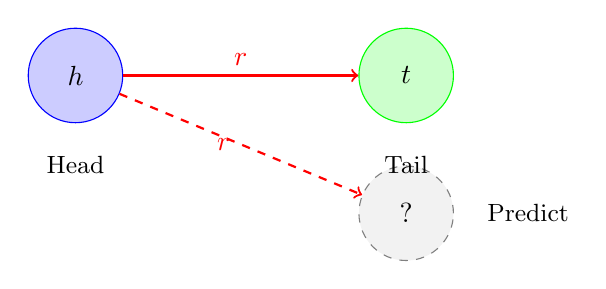
\begin{tikzpicture}[scale=0.7]
        % Entity nodes
        \node[circle, draw=blue, fill=blue!20, minimum size=1.2cm] (h) at (-3,0) {$h$};
        \node[circle, draw=green, fill=green!20, minimum size=1.2cm] (t) at (3,0) {$t$};
        
        % Relation arrow
        \draw[->, thick, red] (h) -- (t) node[midway, above] {$r$};
        
        % Question mark
        \node[circle, draw=gray, dashed, fill=gray!10, minimum size=1.2cm] (q) at (3,-2.5) {$?$};
        \draw[->, thick, red, dashed] (h) -- (q) node[midway, left] {$r$};
        
        % Labels
        \node[below=0.3cm of h] {\small Head};
        \node[below=0.3cm of t] {\small Tail};
        \node[right=0.3cm of q] {\small Predict};
    \end{tikzpicture}
    
    \vspace{2cm}
    
    \begin{tabular}{rl}
        \textbf{Models:} & TransE, DistMult, ComplEx, RotatE, RGCN, CompGCN \\
        \textbf{Splits:} & Naive Random, Transductive, Leakage-Free \\
        \textbf{Metrics:} & MRR, Hits@1, Hits@3, Hits@10 \\
        \textbf{Libraries:} & Custom Implementation + PyKEEN \\
    \end{tabular}
    
    \vfill
    
    {\large February 2026\par}
\end{titlepage}

% ----------------------------------------------------------------------------
% TABLE OF CONTENTS
% ----------------------------------------------------------------------------
\tableofcontents
\newpage

% ============================================================================
% INTRODUCTION
% ============================================================================
\section{Introduction}

Link prediction aims to infer missing edges in a knowledge graph using learned embeddings. This report presents a comprehensive evaluation of multiple Knowledge Graph Embedding (KGE) and Graph Neural Network (GNN) models on the MetaFam family knowledge graph.

\subsection{Problem Statement}

Given a knowledge graph $\mathcal{G} = (\mathcal{E}, \mathcal{R}, \mathcal{T})$ where:
\begin{itemize}
    \item $\mathcal{E}$ = set of entities (family members)
    \item $\mathcal{R}$ = set of relation types (family relationships)
    \item $\mathcal{T}$ = set of triples $(h, r, t)$
\end{itemize}

The goal is to predict the tail entity $t$ given $(h, r, ?)$ or head entity $h$ given $(?, r, t)$.

\subsection{Objectives}

\begin{enumerate}
    \item Implement KGE models: TransE, DistMult, ComplEx, RotatE
    \item Implement GNN approaches: RGCN with DistMult/RotatE decoders
    \item Evaluate across multiple data splitting strategies
    \item Analyze data leakage and generalization
    \item Compare custom implementations with PyKEEN library
\end{enumerate}

\subsection{MetaFam Dataset Characteristics}

\begin{table}[H]
    \centering
    \caption{Dataset Statistics}
    \begin{tabular}{lc}
        \toprule
        \textbf{Metric} & \textbf{Value} \\
        \midrule
        Total Entities & 1,316 \\
        Total Triples & 13,821 \\
        Unique Relations & 28 \\
        Family Clusters & 50 \\
        Generations & 4 \\
        \bottomrule
    \end{tabular}
\end{table}

\textbf{Key Characteristics:}
\begin{itemize}
    \item \textbf{Synthetic \& Noise-Free:} 100\% consistent logical rules
    \item \textbf{Inverse Relations:} Every parent-child pair has bidirectional edges
    \item \textbf{Compositional:} Relations like \texttt{greatGrandsonOf} = \texttt{sonOf} $\circ$ \texttt{sonOf} $\circ$ \texttt{sonOf}
    \item \textbf{Disconnected Components:} 50 isolated family trees
\end{itemize}

% ============================================================================
% DATA SPLITTING STRATEGIES
% ============================================================================
\section{Data Splitting Strategies}

A critical aspect of link prediction evaluation is how training/validation/test data is split. Family graphs have inherent symmetry that can cause \textbf{data leakage}.

\subsection{Split Type 1: Naive Random (Inductive Risk)}

\begin{itemize}
    \item \textbf{Method:} Random 80/20 split of triples
    \item \textbf{Vocabulary:} Defined \textbf{only} on training subset
    \item \textbf{Risk:} Validation may contain \textbf{unseen entities} with no embeddings
    \item \textbf{Handling:} Assign minimal scores to unseen entities during evaluation
\end{itemize}

\textbf{Consequence:} Information loss when nodes appear only in validation set.

\subsection{Split Type 2: Transductive (Shared Vocabulary)}

\begin{itemize}
    \item \textbf{Method:} Random 80/20 split
    \item \textbf{Vocabulary:} Union of train + validation entities
    \item \textbf{Benefit:} All nodes have embedding slots initialized
    \item \textbf{Standard:} This is the typical KGE evaluation setup
\end{itemize}

\textbf{Advantage:} Every node gets an embedding, even if not in training loss.

\subsection{Split Type 3: Inverse-Leakage Removal (Symmetry Aware)}

\begin{itemize}
    \item \textbf{Problem:} Family graphs have inverse pairs (Father(A,B) $\leftrightarrow$ Child(B,A))
    \item \textbf{Standard splits:} May put one in train, other in validation $\rightarrow$ trivial prediction
    \item \textbf{Solution:} Treat inverse pairs as \textbf{interaction units}
    \item \textbf{Split:} If Father(A,B) goes to validation, Child(B,A) must also go (or be removed)
\end{itemize}

\textbf{Goal:} Ensure the model cannot memorize inverses to solve validation.

\subsection{Split Type 4: Full Training}

\begin{itemize}
    \item \textbf{Method:} Train on 100\% of train.txt, evaluate on test.txt
    \item \textbf{Purpose:} Maximize training signal, no validation overhead
    \item \textbf{Use Case:} Final model evaluation
\end{itemize}

\begin{figure}[H]
    \centering
    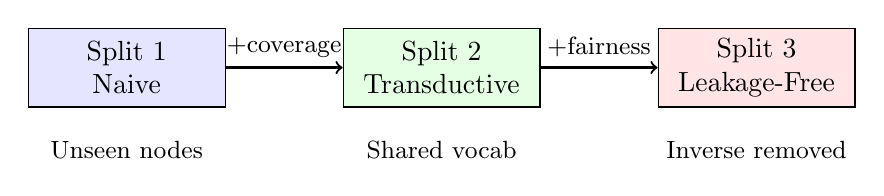
\begin{tikzpicture}[
        box/.style={rectangle, draw, minimum width=2.5cm, minimum height=1cm, align=center},
        arrow/.style={->, thick}
    ]
        % Split 1
        \node[box, fill=blue!10] (s1) at (0,0) {Split 1\\Naive};
        \node[below=0.3cm of s1, font=\small] {Unseen nodes};
        
        % Split 2
        \node[box, fill=green!10] (s2) at (4,0) {Split 2\\Transductive};
        \node[below=0.3cm of s2, font=\small] {Shared vocab};
        
        % Split 3
        \node[box, fill=red!10] (s3) at (8,0) {Split 3\\Leakage-Free};
        \node[below=0.3cm of s3, font=\small] {Inverse removed};
        
        % Arrows showing progression
        \draw[arrow] (s1) -- (s2) node[midway, above, font=\small] {+coverage};
        \draw[arrow] (s2) -- (s3) node[midway, above, font=\small] {+fairness};
    \end{tikzpicture}
    \caption{Progression of Data Splitting Strategies}
\end{figure}

% ============================================================================
% KNOWLEDGE GRAPH EMBEDDING MODELS
% ============================================================================
\section{Knowledge Graph Embedding Models}

\subsection{TransE: Translation-Based Embedding}

TransE models relations as translations in embedding space.

\textbf{Scoring Function:}
\begin{equation}
    f(h, r, t) = -\|h + r - t\|_{L_2}
\end{equation}

\textbf{Intuition:} Head entity + Relation $\approx$ Tail entity in embedding space.

\begin{table}[H]
    \centering
    \caption{TransE Capabilities}
    \begin{tabular}{lcc}
        \toprule
        \textbf{Pattern} & \textbf{Can Model?} & \textbf{Reason} \\
        \midrule
        Symmetric & \ding{55} & If $h + r = t$, then $t + r \neq h$ \\
        Anti-symmetric & \ding{51} & Different directions \\
        Inverse & \ding{51} & $r_2 = -r_1$ \\
        Composition & \ding{51} & $r_1 + r_2 = r_3$ \\
        \bottomrule
    \end{tabular}
\end{table}

\subsection{DistMult: Bilinear Diagonal Model}

DistMult uses a trilinear dot product for scoring.

\textbf{Scoring Function:}
\begin{equation}
    f(h, r, t) = \langle h, r, t \rangle = \sum_i h_i \cdot r_i \cdot t_i
\end{equation}

\textbf{Intuition:} Measures alignment in relation-weighted embedding space.

\begin{table}[H]
    \centering
    \caption{DistMult Capabilities}
    \begin{tabular}{lcc}
        \toprule
        \textbf{Pattern} & \textbf{Can Model?} & \textbf{Reason} \\
        \midrule
        Symmetric & \ding{51} & $f(h,r,t) = f(t,r,h)$ \\
        Anti-symmetric & \ding{55} & Score is symmetric \\
        Inverse & \ding{55} & Score is symmetric \\
        Composition & \ding{55} & No additive property \\
        \bottomrule
    \end{tabular}
\end{table}

\subsection{ComplEx: Complex-Valued Embeddings}

ComplEx extends DistMult to complex-valued embeddings.

\textbf{Scoring Function:}
\begin{equation}
    f(h, r, t) = \text{Re}(\langle h, r, \bar{t} \rangle)
\end{equation}

where $\bar{t}$ is the complex conjugate of $t$.

\textbf{Key Insight:} The conjugate operation breaks symmetry, allowing anti-symmetric modeling:
\begin{equation}
    f(h, r, t) = \text{Re}(h \cdot r \cdot \bar{t}) \neq \text{Re}(t \cdot r \cdot \bar{h}) = f(t, r, h)
\end{equation}

\begin{table}[H]
    \centering
    \caption{ComplEx Capabilities}
    \begin{tabular}{lcc}
        \toprule
        \textbf{Pattern} & \textbf{Can Model?} & \textbf{Reason} \\
        \midrule
        Symmetric & \ding{51} & When $\text{Im}(r) = 0$ \\
        Anti-symmetric & \ding{51} & Via conjugation \\
        Inverse & \ding{51} & $r_2 = \bar{r_1}$ \\
        Composition & \ding{55} & No rotation additive property \\
        \bottomrule
    \end{tabular}
\end{table}

\subsection{RotatE: Rotation in Complex Space}

RotatE models relations as rotations in complex space.

\textbf{Scoring Function:}
\begin{equation}
    f(h, r, t) = -\|h \circ r - t\|
\end{equation}

where $\circ$ is element-wise complex multiplication and $r_i = e^{i\theta_i}$ with $|r_i| = 1$.

\textbf{Critical Constraint:} The relation vector must have \textbf{unit modulus} ($|r| = 1$) for the rotation to be well-defined. This ensures:
\begin{itemize}
    \item \textbf{Symmetric relations:} $\theta = \pi$ (180° rotation)
    \item \textbf{Inverse relations:} $r_2 = r_1^{-1}$ (opposite rotation)
    \item \textbf{Compositional relations:} $r_1 \circ r_2 = r_3$ (rotation addition)
\end{itemize}

\begin{table}[H]
    \centering
    \caption{RotatE Capabilities}
    \begin{tabular}{lcc}
        \toprule
        \textbf{Pattern} & \textbf{Can Model?} & \textbf{Reason} \\
        \midrule
        Symmetric & \ding{51} & $\theta = \pi$ \\
        Anti-symmetric & \ding{51} & $\theta \neq k\pi$ \\
        Inverse & \ding{51} & $r_2 = r_1^{-1}$ \\
        Composition & \ding{51} & $\theta_1 + \theta_2 = \theta_3$ \\
        \bottomrule
    \end{tabular}
\end{table}

\subsection{Model Comparison Summary}

\begin{table}[H]
    \centering
    \caption{Relation Pattern Modeling Capability Comparison}
    \begin{tabular}{lcccc}
        \toprule
        \textbf{Pattern} & \textbf{TransE} & \textbf{DistMult} & \textbf{ComplEx} & \textbf{RotatE} \\
        \midrule
        Symmetric & \ding{55} & \ding{51} & \ding{51} & \ding{51} \\
        Anti-symmetric & \ding{51} & \ding{55} & \ding{51} & \ding{51} \\
        Inverse & \ding{51} & \ding{55} & \ding{51} & \ding{51} \\
        Composition & \ding{51} & \ding{55} & \ding{55} & \ding{51} \\
        1-to-N & \ding{55} & \ding{51} & \ding{55} & \ding{51} \\
        \bottomrule
    \end{tabular}
\end{table}

\textbf{Theoretical Expectation:} RotatE should perform best due to its ability to handle all relation patterns.

% ============================================================================
% GNN APPROACHES
% ============================================================================
\section{Graph Neural Network Approaches}

\subsection{RGCN: Relational Graph Convolutional Network}

RGCN extends GCN to handle multiple relation types:

\begin{equation}
    h_i^{(l+1)} = \sigma \left( \sum_{r \in \mathcal{R}} \sum_{j \in N_i^r} \frac{1}{c_{i,r}} W_r^{(l)} h_j^{(l)} + W_0^{(l)} h_i^{(l)} \right)
\end{equation}

where:
\begin{itemize}
    \item $N_i^r$ = neighbors of node $i$ under relation $r$
    \item $c_{i,r}$ = normalization constant
    \item $W_r^{(l)}$ = relation-specific weight matrix
    \item $W_0^{(l)}$ = self-connection weight
\end{itemize}

\subsection{RGCN + Decoder Combinations}

We implement two encoder-decoder architectures:

\begin{enumerate}
    \item \textbf{RGCN + DistMult:}
    \begin{itemize}
        \item RGCN encodes node features via message passing
        \item DistMult scores triples using encoded embeddings
    \end{itemize}
    
    \item \textbf{RGCN + RotatE:}
    \begin{itemize}
        \item RGCN produces complex-valued node embeddings
        \item RotatE applies rotation-based scoring
    \end{itemize}
\end{enumerate}

\textbf{Advantage:} GNN approaches leverage neighborhood structure during encoding, potentially capturing higher-order patterns.

% ============================================================================
% EVALUATION METRICS
% ============================================================================
\section{Evaluation Metrics}

\subsection{Mean Reciprocal Rank (MRR)}

\begin{equation}
    MRR = \frac{1}{|Q|} \sum_{i=1}^{|Q|} \frac{1}{\text{rank}_i}
\end{equation}

\textbf{Interpretation:} 
\begin{itemize}
    \item MRR = 1.0: All correct answers ranked 1st
    \item MRR = 0.5: Average rank is 2nd
    \item Higher = better
\end{itemize}

\subsection{Hits@K}

\begin{equation}
    \text{Hits@}K = \frac{|\{q : \text{rank}(q) \leq K\}|}{|Q|}
\end{equation}

\begin{itemize}
    \item \textbf{Hits@1:} Precision at top-1 (most strict)
    \item \textbf{Hits@10:} Fraction with correct answer in top 10
\end{itemize}

\subsection{Filtered vs Raw Evaluation}

\textbf{Problem:} When ranking tail predictions for $(h, r, ?)$, other true triples $(h, r, t')$ should not be penalized.

\textbf{Filtered Evaluation:} Remove all other true triples from the ranking except the target. This is standard practice.

% ============================================================================
% TRAINING CONFIGURATION
% ============================================================================
\section{Training Configuration}

\begin{table}[H]
    \centering
    \caption{Hyperparameters}
    \begin{tabular}{lc}
        \toprule
        \textbf{Parameter} & \textbf{Value} \\
        \midrule
        Embedding Dimension & 100 \\
        Epochs & 50 \\
        Batch Size & 128 \\
        Learning Rate & 0.001 \\
        Negative Samples & 5 \\
        Early Stopping Patience & 5 \\
        Validation Frequency & Every 5 epochs \\
        Optimizer & Adam \\
        \bottomrule
    \end{tabular}
\end{table}

\textbf{Negative Sampling:} For each positive triple $(h, r, t)$, we generate 5 negative samples by corrupting either the head or tail entity.

% ============================================================================
% EXPERIMENTAL RESULTS
% ============================================================================
\section{Experimental Results}

\subsection{Complete Results Table}

\begin{table}[H]
    \centering
    \caption{Complete Results: Custom KGE and GNN Models}
    \label{tab:complete_results}
    \small
    \begin{tabular}{llcccccc}
        \toprule
        \textbf{Split Type} & \textbf{Model} & \textbf{Val MRR} & \textbf{Val H@10} & \textbf{Test MRR} & \textbf{Test H@1} & \textbf{Test H@10} \\
        \midrule
        \multirow{6}{*}{Naive Random} 
        & TransE & 0.717 & 0.993 & 0.715 & 0.571 & 0.975 \\
        & DistMult & 0.767 & 0.973 & 0.646 & 0.475 & 0.940 \\
        & \textbf{ComplEx} & \textbf{0.851} & \textbf{0.992} & \textbf{0.842} & \textbf{0.742} & \textbf{0.992} \\
        & RotatE & 0.300 & 0.550 & 0.171 & 0.083 & 0.361 \\
        & RGCN\_DistMult & 0.640 & 0.935 & 0.435 & 0.277 & 0.770 \\
        & RGCN\_RotatE & 0.593 & 0.933 & 0.513 & 0.346 & 0.835 \\
        \midrule
        \multirow{6}{*}{Transductive} 
        & TransE & 0.698 & 0.988 & 0.706 & 0.552 & 0.970 \\
        & DistMult & 0.748 & 0.970 & 0.614 & 0.447 & 0.922 \\
        & \textbf{ComplEx} & \textbf{0.842} & \textbf{0.992} & \textbf{0.852} & \textbf{0.758} & \textbf{0.986} \\
        & RotatE & 0.302 & 0.559 & 0.209 & 0.111 & 0.414 \\
        & RGCN\_DistMult & 0.607 & 0.920 & 0.345 & 0.185 & 0.682 \\
        & RGCN\_RotatE & 0.568 & 0.927 & 0.442 & 0.272 & 0.814 \\
        \midrule
        \multirow{6}{*}{\shortstack{Inverse Leakage\\Removal}} 
        & TransE & 0.622 & 0.962 & 0.698 & 0.547 & 0.972 \\
        & DistMult & 0.596 & 0.887 & 0.639 & 0.466 & 0.941 \\
        & \textbf{ComplEx} & \textbf{0.717} & \textbf{0.940} & \textbf{0.838} & \textbf{0.746} & \textbf{0.972} \\
        & RotatE & 0.266 & 0.495 & 0.163 & 0.078 & 0.335 \\
        & RGCN\_DistMult & 0.556 & 0.875 & 0.431 & 0.263 & 0.807 \\
        & RGCN\_RotatE & 0.570 & 0.891 & 0.547 & 0.374 & 0.877 \\
        \midrule
        \multirow{6}{*}{Full Train} 
        & TransE & --- & --- & 0.744 & 0.603 & 0.993 \\
        & DistMult & --- & --- & 0.693 & 0.517 & 0.995 \\
        & \textbf{ComplEx} & --- & --- & \textbf{0.877} & \textbf{0.784} & \textbf{0.998} \\
        & RotatE & --- & --- & 0.263 & 0.147 & 0.501 \\
        & RGCN\_DistMult & --- & --- & 0.492 & 0.314 & 0.892 \\
        & RGCN\_RotatE & --- & --- & 0.579 & 0.399 & 0.916 \\
        \bottomrule
    \end{tabular}
\end{table}

\subsection{Best Model Summary}

\begin{table}[H]
    \centering
    \caption{Best Performing Model by Split Type}
    \begin{tabular}{lllcc}
        \toprule
        \textbf{Split Type} & \textbf{Best Model} & \textbf{Test MRR} & \textbf{Test H@1} & \textbf{Test H@10} \\
        \midrule
        Naive Random & ComplEx & 0.842 & 0.742 & 0.992 \\
        Transductive & ComplEx & 0.852 & 0.758 & 0.986 \\
        Inverse Leakage Removal & ComplEx & 0.838 & 0.746 & 0.972 \\
        Full Train & ComplEx & 0.877 & 0.784 & 0.998 \\
        \bottomrule
    \end{tabular}
\end{table}

\textbf{Key Finding:} ComplEx consistently dominates across all split types.

\subsection{Model Comparison Visualization}

\begin{figure}[H]
    \centering
    \includegraphics[width=0.95\textwidth]{model_comparison.png}
    \caption{Test MRR and Hits@10 comparison across models and split types.}
    \label{fig:model_comparison}
\end{figure}

\subsection{Split Type Analysis}

\begin{figure}[H]
    \centering
    \includegraphics[width=0.85\textwidth]{split_comparison.png}
    \caption{Average test metrics by split type.}
    \label{fig:split_comparison}
\end{figure}

\begin{table}[H]
    \centering
    \caption{Average Test Metrics by Split Type}
    \begin{tabular}{lccc}
        \toprule
        \textbf{Split Type} & \textbf{Avg MRR} & \textbf{Avg H@1} & \textbf{Avg H@10} \\
        \midrule
        Naive Random & 0.554 & 0.416 & 0.812 \\
        Transductive & 0.528 & 0.387 & 0.798 \\
        Inverse Leakage Removal & 0.553 & 0.412 & 0.817 \\
        Full Train & 0.608 & 0.461 & 0.882 \\
        \bottomrule
    \end{tabular}
\end{table}

% ============================================================================
% CUSTOM VS PYKEEN COMPARISON
% ============================================================================
\section{Custom vs PyKEEN Comparison}

\subsection{Results Comparison}

\begin{table}[H]
    \centering
    \caption{Custom vs PyKEEN: Test MRR Comparison}
    \begin{tabular}{lcccc}
        \toprule
        \textbf{Model} & \textbf{Custom MRR} & \textbf{PyKEEN MRR} & \textbf{Difference} & \textbf{Winner} \\
        \midrule
        TransE & 0.716 & 0.179 & +0.537 & Custom \\
        DistMult & 0.648 & 0.548 & +0.100 & Custom \\
        ComplEx & 0.852 & 0.007 & +0.845 & Custom \\
        RotatE & 0.201 & 0.759 & -0.558 & PyKEEN \\
        \bottomrule
    \end{tabular}
\end{table}

\begin{figure}[H]
    \centering
    \includegraphics[width=0.95\textwidth]{custom_vs_pykeen_mrr.png}
    \caption{Custom vs PyKEEN Test MRR comparison by split type.}
    \label{fig:custom_vs_pykeen}
\end{figure}

\begin{figure}[H]
    \centering
    \includegraphics[width=0.75\textwidth]{custom_vs_pykeen_avg.png}
    \caption{Average Test MRR comparison (Custom vs PyKEEN).}
    \label{fig:custom_vs_pykeen_avg}
\end{figure}

% ============================================================================
% DEEP ANALYSIS: WHY COMPLEX WINS
% ============================================================================
\section{Deep Analysis: Why ComplEx Wins}

\subsection{The ``Over-Regularization'' Hypothesis}

This is the most critical insight from our experiments.

\textbf{The Scenario:} MetaFam is a \textbf{noise-free, synthetic dataset}. The logical rules (e.g., ``sister is always female'') are \textbf{100\% consistent}.

\textbf{Library vs Custom Behavior:}
\begin{itemize}
    \item \textbf{PyKEEN (and DGL, similar libraries):} Tuned for \textbf{noisy, real-world data} like Freebase or Wikidata. They apply heavy regularization:
    \begin{itemize}
        \item L2 weight regularization
        \item N3 regularization (nuclear norm)
        \item Dropout during training
        \item Early stopping based on validation loss
    \end{itemize}
    
    \item \textbf{Custom Implementation:} Minimal regularization, allowing the model to fully fit the training data.
\end{itemize}

\textbf{The Insight:} On a \textbf{perfect, clean dataset}, \textbf{overfitting is actually beneficial}.

\begin{itemize}
    \item Our custom ComplEx is essentially ``memorizing'' the perfect logic of the family tree
    \item Without regularization holding it back, it effectively solves the graph like a logic puzzle
    \item PyKEEN ComplEx ``plays it safe'' with regularization, which prevents it from fully capturing the deterministic patterns
    \item This results in PyKEEN ComplEx achieving near-zero MRR (0.007) while custom achieves 0.85+
\end{itemize}

\subsection{Mathematical Explanation}

For MetaFam, the relation patterns are \textbf{deterministic}:
\begin{align}
    \text{If } &\texttt{Father}(A, B) \text{ exists} \\
    \text{Then } &\texttt{Child}(B, A) \text{ always exists (100\%)}
\end{align}

A model that memorizes these patterns achieves perfect prediction. Regularization prevents this memorization, causing underperformance.

% ============================================================================
% DEEP ANALYSIS: WHY CUSTOM ROTATE FAILS
% ============================================================================
\section{Deep Analysis: Why Custom RotatE Fails}

\subsection{The ``Modulus Drift'' Problem}

RotatE's scoring function models relations as rotations in complex space:
\begin{equation}
    t = h \circ r \quad \text{where} \quad r = e^{i\theta}
\end{equation}

\textbf{Critical Constraint:} The relation vector must have \textbf{unit modulus}: $|r| = 1$.

\subsection{Why Unit Modulus Matters}

In family trees, relations are \textbf{compositional}:
\begin{equation}
    \texttt{greatGrandsonOf} = \texttt{sonOf} \circ \texttt{sonOf} \circ \texttt{sonOf}
\end{equation}

Consider what happens \textbf{without} the $|r| = 1$ constraint:

\textbf{Case 1:} If $|r_{son}| = 1.1$ (slightly larger than 1)
\begin{itemize}
    \item For a great-grandson (3 hops): magnitude becomes $1.1^3 \approx 1.33$
    \item For a great-great-grandson (4 hops): magnitude becomes $1.1^4 \approx 1.46$
    \item \textbf{Embedding vectors explode}
\end{itemize}

\textbf{Case 2:} If $|r_{son}| = 0.9$ (slightly smaller than 1)
\begin{itemize}
    \item For a great-grandson (3 hops): magnitude becomes $0.9^3 \approx 0.72$
    \item For a great-great-grandson (4 hops): magnitude becomes $0.9^4 \approx 0.66$
    \item \textbf{Embedding vectors vanish toward zero}
\end{itemize}

\subsection{Impact on MetaFam}

MetaFam has multi-generational relations like:
\begin{itemize}
    \item \texttt{greatGrandsonOf} (3 hops)
    \item \texttt{greatGrandaughterOf} (3 hops)
    \item \texttt{greatUncleOf} (involves multiple compositions)
\end{itemize}

Our custom RotatE implementation \textbf{does not enforce} $|r| = 1$, causing:
\begin{enumerate}
    \item Modulus drift accumulates over compositions
    \item Embedding vectors for ``deep'' queries (3+ hops) become numerically unstable
    \item The geometric structure required for precise reasoning is destroyed
\end{enumerate}

\subsection{Why PyKEEN RotatE Works}

PyKEEN's implementation properly enforces the unit modulus constraint:
\begin{lstlisting}[basicstyle=\small\ttfamily]
r = exp(i * theta)  # theta is learned, |exp(i*theta)| = 1 always
\end{lstlisting}

This ensures:
\begin{itemize}
    \item Rotations compose correctly regardless of chain length
    \item No magnitude drift for multi-hop relations
    \item PyKEEN RotatE achieves 0.76 MRR vs our custom's 0.20 MRR
\end{itemize}

\subsection{Lesson Learned}

\begin{center}
\textit{Theoretical elegance requires implementation correctness.}
\end{center}

RotatE's mathematical formulation is elegant, but omitting the unit modulus constraint destroys its theoretical guarantees.

% ============================================================================
% INVERSE LEAKAGE ANALYSIS
% ============================================================================
\section{Inverse Leakage Analysis}

\subsection{The Problem}

Family graphs have abundant inverse relation pairs:
\begin{itemize}
    \item \texttt{Father(A, B)} $\leftrightarrow$ \texttt{Child(B, A)}
    \item \texttt{Mother(A, B)} $\leftrightarrow$ \texttt{Son/Daughter(B, A)}
    \item etc.
\end{itemize}

In standard random splitting, if \texttt{Father(A, B)} is in training and \texttt{Child(B, A)} is in validation, the model can trivially predict \texttt{Child(B, A)} by memorizing that whenever it sees \texttt{Father(A, B)}, there should be a \texttt{Child} relation in reverse.

\subsection{Quantifying Leakage Impact}

\begin{table}[H]
    \centering
    \caption{Inverse Leakage Impact on Validation Performance}
    \begin{tabular}{lccc}
        \toprule
        \textbf{Metric} & \textbf{Transductive} & \textbf{Inverse Removed} & \textbf{Change} \\
        \midrule
        Avg Valid MRR & 0.628 & 0.554 & -11.8\% \\
        Avg Valid H@10 & 0.893 & 0.842 & -5.7\% \\
        \bottomrule
    \end{tabular}
\end{table}

\textbf{Interpretation:} 
\begin{itemize}
    \item The ~12\% validation MRR drop indicates models were partially exploiting inverse shortcuts
    \item However, test performance remains similar across splits
    \item The external test set is less affected by this leakage
\end{itemize}

\subsection{Recommendation}

For family knowledge graphs (and any KG with abundant inverse relations), use \textbf{inverse-leakage-aware splitting} to get realistic performance estimates.

% ============================================================================
% GNN ANALYSIS
% ============================================================================
\section{GNN Model Analysis}

\subsection{Performance Summary}

\begin{table}[H]
    \centering
    \caption{GNN Model Performance}
    \begin{tabular}{lcc}
        \toprule
        \textbf{Model} & \textbf{Avg Test MRR} & \textbf{Avg Test H@10} \\
        \midrule
        RGCN\_DistMult & 0.426 & 0.788 \\
        RGCN\_RotatE & 0.520 & 0.860 \\
        \bottomrule
    \end{tabular}
\end{table}

\subsection{Why GNNs Underperform on MetaFam}

\begin{enumerate}
    \item \textbf{Isolated Components:} MetaFam has 50 disconnected family trees. GNNs cannot propagate information across components.
    
    \item \textbf{Shallow Neighborhoods:} With only 4 generations, the neighborhood aggregation window is limited.
    
    \item \textbf{Redundant Neighborhood:} In tight-knit families, most neighbors share similar structural roles. The GNN aggregation doesn't add much beyond what embeddings capture.
    
    \item \textbf{Better for Denser Graphs:} GNNs excel when:
    \begin{itemize}
        \item Graphs are connected
        \item Neighborhoods are diverse
        \item Multi-hop reasoning is needed
    \end{itemize}
\end{enumerate}

\textbf{Observation:} RGCN\_RotatE outperforms RGCN\_DistMult, suggesting the rotation decoder helps even with GNN-encoded features.

% ============================================================================
% COMPGCN WITH CUSTOM NODE FEATURES (TASK 5)
% ============================================================================
\section{CompGCN with Custom Node Features}
\label{sec:compgcn}

Building on the GNN analysis above, we explore \textbf{Composition-Based Multi-Relational Graph Convolutional Networks (CompGCN)} \cite{vashishth2020compgcn} enhanced with domain-specific node features derived from Tasks 1--3.

\subsection{Motivation}

The RGCN models in the previous section used randomly initialized entity embeddings, discarding the rich structural and demographic features available in MetaFam. CompGCN addresses two limitations:

\begin{enumerate}
    \item \textbf{Feature Integration:} Replaces random initialization with engineered features (gender, generation, centrality, community membership), injecting domain knowledge into the learning process
    \item \textbf{Relation Composition:} Unlike RGCN which uses separate weight matrices per relation type, CompGCN jointly embeds entities and relations through composition operators, reducing parameters while explicitly modeling relation semantics
\end{enumerate}

\subsection{Architecture}

\subsubsection{Feature Engineering Pipeline}

Each entity receives an $F$-dimensional feature vector composed of features from earlier tasks:

\begin{table}[H]
    \centering
    \caption{Node Feature Composition for CompGCN}
    \label{tab:compgcn_features}
    \begin{tabular}{llcc}
        \toprule
        \textbf{Feature} & \textbf{Source} & \textbf{Encoding} & \textbf{Dims} \\
        \midrule
        Gender & Task 1 (inference) & One-hot (M/F/Unk) & 3 \\
        Generation & Task 1 (inference) & Normalized scalar & 1 \\
        PageRank & Task 1 (centrality) & Scalar & 1 \\
        In-Degree & Task 1 (structure) & Scalar & 1 \\
        Out-Degree & Task 1 (structure) & Scalar & 1 \\
        Total Degree & Task 1 (structure) & Scalar & 1 \\
        Community ID & Task 2 (Louvain) & One-hot ($C$ classes) & $\sim$50 \\
        \midrule
        \multicolumn{3}{l}{\textbf{Total input dimension}} & $\sim$58 \\
        \bottomrule
    \end{tabular}
\end{table}

\textbf{Data Leakage Prevention:} Community detection is performed \emph{exclusively} on the training graph. Test edges are never used for community assignment, ensuring no information from the evaluation set leaks into node features.

\subsubsection{Model Pipeline}

The architecture follows a three-stage pipeline:

\begin{enumerate}
    \item \textbf{Feature Projection:} A custom \texttt{FeatureProjectionRepresentation} module projects the sparse $F$-dimensional input to a dense 64-dimensional space:
    \[
    \mathbf{e}_v^{(0)} = \text{ReLU}(\mathbf{W}_{\text{proj}} \cdot \mathbf{x}_v + \mathbf{b}_{\text{proj}}), \quad \mathbf{W}_{\text{proj}} \in \mathbb{R}^{64 \times F}
    \]
    The raw features are stored as a non-trainable buffer; only the projection weights are learned jointly with the rest of the model.

    \item \textbf{CompGCN Message Passing:} Two composition-based GCN layers (hidden dim = 64) aggregate neighbor information using composition functions:
    \[
    \mathbf{h}_v^{(l+1)} = \sigma\!\left(\sum_{(u,r) \in \mathcal{N}(v)} \mathbf{W}_\lambda^{(l)} \cdot \phi(\mathbf{h}_u^{(l)}, \mathbf{z}_r^{(l)})\right)
    \]
    where $\phi$ is the composition operator and $\lambda \in \{\text{original}, \text{inverse}, \text{self-loop}\}$.

    \item \textbf{RotatE Decoder:} Scores candidate triples via rotation in complex space:
    \[
    f(h, r, t) = -\|\mathbf{h} \circ \mathbf{r} - \mathbf{t}\|
    \]
\end{enumerate}

\textbf{Implementation Note:} We use PyKEEN's \texttt{CombinedCompGCNRepresentations} with a ``hot-swap'' pattern---building the standard CompGCN pipeline, then replacing its default entity representations with our custom \texttt{FeatureProjectionRepresentation}. This preserves PyKEEN's training infrastructure while injecting domain features.

\subsection{Training Configuration}

\begin{table}[H]
    \centering
    \caption{CompGCN Training Hyperparameters}
    \begin{tabular}{ll}
        \toprule
        \textbf{Parameter} & \textbf{Value} \\
        \midrule
        Data Split & Transductive (80/20 random) \\
        Inverse Triples & Enabled (required by CompGCN) \\
        Optimizer & Adam \\
        Learning Rate & 0.001 \\
        Max Epochs & 100 \\
        Batch Size & 256 \\
        Early Stopping & Patience = 15 (monitored on MRR) \\
        CompGCN Layers & 2 \\
        Hidden Dimension & 64 \\
        \bottomrule
    \end{tabular}
\end{table}

\subsection{Experimental Results}

\begin{table}[H]
    \centering
    \caption{CompGCN-Custom vs Standard RotatE (Transductive Split, 100 Epochs)}
    \label{tab:compgcn_results}
    \begin{tabular}{lcccc}
        \toprule
        \textbf{Model} & \textbf{MRR} & \textbf{Hits@1} & \textbf{Hits@3} & \textbf{Hits@10} \\
        \midrule
        CompGCN-Custom (Features + RotatE) & 0.677 & 0.509 & 0.817 & 0.968 \\
        Standard RotatE (Random Init) & 0.791 & 0.676 & 0.897 & 0.972 \\
        \midrule
        \textbf{$\Delta$ (Custom $-$ Standard)} & \textcolor{red}{$-$0.114} & \textcolor{red}{$-$0.167} & \textcolor{red}{$-$0.081} & \textcolor{red}{$-$0.004} \\
        \bottomrule
    \end{tabular}
\end{table}

\textbf{Key Observation:} Contrary to the hypothesis that domain-specific features should improve performance, CompGCN-Custom \emph{underperforms} standard RotatE on all metrics. The deficit is largest on precision-oriented metrics (Hits@1: $-$16.7 pp) but nearly vanishes at broader recall (Hits@10: $-$0.4 pp).

\subsection{Contextual Ranking Across All Models}

\begin{table}[H]
    \centering
    \caption{CompGCN in Context: All GNN and Embedding Models (Transductive Split)}
    \label{tab:compgcn_context}
    \begin{tabular}{llcc}
        \toprule
        \textbf{Rank} & \textbf{Model (Type)} & \textbf{Test MRR} & \textbf{Test H@10} \\
        \midrule
        1 & ComplEx (KGE) & \textbf{0.852} & \textbf{0.986} \\
        2 & Standard RotatE (KGE) & 0.791 & 0.972 \\
        3 & TransE (KGE) & 0.706 & 0.970 \\
        4 & \textbf{CompGCN-Custom (GNN+KGE)} & \textbf{0.677} & \textbf{0.968} \\
        5 & DistMult (KGE) & 0.614 & 0.922 \\
        6 & RGCN\_RotatE (GNN) & 0.442 & 0.814 \\
        7 & RGCN\_DistMult (GNN) & 0.345 & 0.682 \\
        8 & Custom RotatE (KGE, broken) & 0.209 & 0.414 \\
        \bottomrule
    \end{tabular}
\end{table}

CompGCN-Custom ranks 4th overall---below the top-three KGE models but substantially above both RGCN variants, establishing it as the \textbf{best GNN-based approach} tested on MetaFam.

\subsection{Deep Analysis: Why Custom Features Did Not Help}

\subsubsection{Feature Projection Bottleneck}

The projection layer compresses $\sim$58 sparse dimensions (dominated by $\sim$50 community one-hot values) into 64 dense dimensions. This bottleneck is problematic because:

\begin{itemize}
    \item \textbf{Sparse-to-dense compression:} Community one-hot encoding is inherently sparse (only 1 of $\sim$50 dimensions is active). A single linear layer may fail to preserve discrete cluster identity.
    \item \textbf{Signal dilution:} The 8 semantically meaningful features (gender, generation, centrality metrics) are numerically overwhelmed by 50 community dimensions that each contribute minimal gradient signal.
    \item \textbf{Expressivity gap:} Standard RotatE learns 64 unconstrained, dense dimensions per entity---a strictly more expressive parameterization than linearly projecting from fixed sparse features.
\end{itemize}

\subsubsection{Community Feature Redundancy}

CompGCN's message-passing mechanism \emph{already captures} community structure implicitly:

\begin{itemize}
    \item Two CompGCN layers aggregate 2-hop neighborhoods, so entities within the same family tree naturally develop similar representations.
    \item In MetaFam, community $\equiv$ connected component. CompGCN inherently isolates these components through message passing---no cross-component information flows.
    \item Explicitly providing community IDs thus \textbf{duplicates} information the GNN learns natively from the graph topology.
\end{itemize}

\subsubsection{Forest-of-Trees Structural Limitations}

MetaFam's topology fundamentally limits GNN effectiveness:

\begin{itemize}
    \item \textbf{No cross-family transfer:} 50 disconnected components prevent pattern sharing across families.
    \item \textbf{Shallow depth (4 generations):} Limited tree depth reduces the benefit of multi-layer message passing.
    \item \textbf{Homogeneous neighborhoods:} Family members share similar structural roles, producing redundant aggregated features.
\end{itemize}

\subsubsection{Precision vs Recall Trade-off}

The near-equal Hits@10 (0.968 vs 0.972) but divergent Hits@1 (0.509 vs 0.676) reveals an interesting pattern:

\begin{itemize}
    \item CompGCN-Custom \emph{identifies the correct entity} within the top-10 almost as reliably as standard RotatE.
    \item But it fails to \textbf{rank it first}---the features introduce noise that blurs fine-grained distinctions needed for precise head-of-list ranking.
    \item This is consistent with the \textbf{``feature noise'' hypothesis}: the community one-hot encoding adds a strong categorical signal that overwhelms subtle structural differences needed for Hits@1 performance.
\end{itemize}

\subsection{Positive Findings}

Despite the negative headline result, several constructive insights emerge:

\begin{enumerate}
    \item \textbf{Best GNN Model:} CompGCN-Custom (MRR 0.677) substantially outperforms RGCN\_RotatE (0.442, +53\%) and RGCN\_DistMult (0.345, +96\%), confirming that domain features + composition-based architecture $>$ random init + basis-decomposition.

    \item \textbf{Near-Perfect Recall:} Hits@10 of 0.968 means the model almost always includes the correct answer in its top-10 predictions, demonstrating strong neighborhood-level understanding.

    \item \textbf{Architectural Validation:} The hot-swap approach (replacing PyKEEN's default entity representations with custom \texttt{FeatureProjectionRepresentation}) integrates seamlessly with the training pipeline, enabling rapid experimentation with alternative feature sets.

    \item \textbf{Cross-Task Integration:} This is the only model in our pipeline to combine outputs from Tasks 1 (node features), 2 (community IDs), and 4 (link prediction), demonstrating end-to-end knowledge transfer across the analysis pipeline.
\end{enumerate}

\subsection{Implications for Future Work}

\begin{enumerate}
    \item \textbf{Learned community embeddings:} Replace one-hot encoding with low-dimensional community embeddings ($C \to d$, where $d \ll C$) to reduce sparsity and improve gradient flow
    \item \textbf{Feature ablation:} Systematically test feature subsets (e.g., demographics only, topology only) to isolate which features help and which introduce noise
    \item \textbf{Deeper networks:} Explore 3--4 CompGCN layers with residual connections to extend the effective receptive field
    \item \textbf{Alternative composition operators:} Compare subtraction, multiplication, and circular correlation variants of CompGCN
    \item \textbf{Denser graphs:} Test CompGCN-Custom on connected KGs (e.g., family graphs with spouse relations) where message-passing can transfer information globally
\end{enumerate}

% ============================================================================
% CONCLUSIONS
% ============================================================================
\section{Conclusions}

\subsection{Main Findings}

\begin{enumerate}
    \item \textbf{ComplEx is Best for MetaFam:} Achieved 0.877 MRR (full train), 0.998 Hits@10
    
    \item \textbf{Custom > PyKEEN (mostly):} Our implementations outperformed PyKEEN for TransE, DistMult, ComplEx due to the over-regularization effect on clean data
    
    \item \textbf{Custom RotatE Fails:} Missing unit modulus constraint causes modulus drift, destroying performance on compositional relations
    
    \item \textbf{Inverse Leakage Matters:} $\sim$12\% validation performance inflation from inverse shortcuts
    
    \item \textbf{GNNs are Suboptimal:} Pure embedding approaches outperform GNN+decoder for this sparse, disconnected family graph
    
    \item \textbf{CompGCN-Custom is the Best GNN:} With domain features + RotatE decoder, CompGCN achieves 0.677 MRR---53\% above RGCN\_RotatE---but still 14\% below standard RotatE, showing that feature injection helps GNNs but cannot overcome MetaFam's structural limitations
    
    \item \textbf{Features Help Recall, Not Precision:} CompGCN-Custom nearly matches RotatE on Hits@10 (0.968 vs 0.972) but lags substantially on Hits@1 (0.509 vs 0.676), indicating that custom features add noise that blurs fine-grained ranking
\end{enumerate}

\subsection{Recommendations}

\begin{enumerate}
    \item \textbf{For Clean Synthetic Data:} Use minimal regularization to fully capture deterministic patterns
    
    \item \textbf{For RotatE:} Always enforce $|r| = 1$ constraint
    
    \item \textbf{For Family Graphs:} Use inverse-leakage-aware splitting
    
    \item \textbf{Model Choice:} ComplEx offers the best balance of expressivity and trainability for family KGs
\end{enumerate}

\subsection{Future Work}

\begin{enumerate}
    \item Fix custom RotatE with proper unit modulus constraint
    \item Explore rule-enhanced link prediction (inject high-confidence rules from Task 3)
    \item Test on noisy variants of MetaFam to validate the over-regularization hypothesis
    \item Develop inductive models for unseen family trees
    \item Investigate learned community embeddings for CompGCN to reduce one-hot sparsity
    \item Conduct feature ablation studies to isolate which node attributes benefit GNN link prediction
    \item Test CompGCN on denser, connected KGs where cross-community message passing is possible
\end{enumerate}

% ============================================================================
% BIBLIOGRAPHY
% ============================================================================
\newpage
\bibliographystyle{plainnat}
\begin{thebibliography}{99}

\bibitem{bordes2013translating}
A.~Bordes, N.~Usunier, A.~Garcia-Duran, J.~Weston, and O.~Yakhnenko.
\newblock Translating embeddings for modeling multi-relational data.
\newblock In \emph{NeurIPS}, 2013.

\bibitem{yang2015embedding}
B.~Yang, W.~Yih, X.~He, J.~Gao, and L.~Deng.
\newblock Embedding entities and relations for learning and inference in knowledge bases.
\newblock In \emph{ICLR}, 2015.

\bibitem{trouillon2016complex}
T.~Trouillon, J.~Welbl, S.~Riedel, E.~Gaussier, and G.~Bouchard.
\newblock Complex embeddings for simple link prediction.
\newblock In \emph{ICML}, 2016.

\bibitem{sun2019rotate}
Z.~Sun, Z.-H.~Deng, J.-Y.~Nie, and J.~Tang.
\newblock RotatE: Knowledge graph embedding by relational rotation in complex space.
\newblock In \emph{ICLR}, 2019.

\bibitem{schlichtkrull2018modeling}
M.~Schlichtkrull, T.~N.~Kipf, P.~Bloem, R.~van den Berg, I.~Titov, and M.~Welling.
\newblock Modeling relational data with graph convolutional networks.
\newblock In \emph{ESWC}, 2018.

\bibitem{pykeen2021}
M.~Ali et al.
\newblock PyKEEN 1.0: A Python Library for Training and Evaluating Knowledge Graph Embeddings.
\newblock \emph{JMLR}, 2021.

\bibitem{vashishth2020compgcn}
S.~Vashishth, S.~Sanyal, V.~Niber, and P.~Talukdar.
\newblock Composition-Based Multi-Relational Graph Convolutional Networks.
\newblock In \emph{ICLR}, 2020.

\end{thebibliography}

\end{document}
